\documentclass[a4paper,12pt,oneside]{book}

%-------------------------------Start of the Preable------------------------------------------------
\usepackage[english]{babel}
\usepackage{blindtext}
%packagr for hyperlinks
\usepackage{hyperref}
\hypersetup{
    colorlinks=true,
    linkcolor=blue,
    filecolor=magenta,      
    urlcolor=cyan,
}

\urlstyle{same}
%use of package fancy header
\usepackage{fancyhdr}
\setlength\headheight{26pt}
\fancyhf{}
%\rhead{
\includegraphics[width=1cm]{logo}}
\lhead{\rightmark}
\rhead{
\includegraphics[width=1cm]{logo}}
\fancyfoot[RE, RO]{\thepage}
\fancyfoot[CE, CO]{\href{http://www.e-yantra.org}{www.e-yantra.org}}

\pagestyle{fancy}

%use of package for section title formatting
\usepackage{titlesec}
\titleformat{\chapter}
  {\Large\bfseries} % format
  {}                % label
  {0pt}             % sep
  {\huge}           % before-code
 
%use of package tcolorbox for colorful textbox
\usepackage[most]{tcolorbox}
\tcbset{colback=cyan!5!white,colframe=cyan!75!black,halign title = flush center}

\newtcolorbox{mybox}[1]{colback=cyan!5!white,
colframe=cyan!75!black,fonttitle=\bfseries,
title=\textbf{\Large{#1}}}

%use of package marginnote for notes in margin
\usepackage{marginnote}

%use of packgage watermark for pages
%\usepackage{draftwatermark}
%\SetWatermarkText{
\includegraphics{logo}}
\usepackage[scale=2,opacity=0.1,angle=0]{background}
\backgroundsetup{
contents={
\includegraphics{logo}}
}

%use of newcommand for keywords color
\usepackage{xcolor}
\newcommand{\keyword}[1]{\textcolor{red}{\textbf{#1}}}

%package for inserting pictures
\usepackage{graphicx}

%package for highlighting
\usepackage{color,soul}

%new command for table
\newcommand{\head}[1]{\textnormal{\textbf{#1}}}


%----------------------End of the Preamble---------------------------------------


\begin{document}

%---------------------Title Page------------------------------------------------
\begin{titlepage}
\raggedright
{\Large eYSIP2017\\[1cm]}
{\Huge\scshape Model Based Design using Statecharts and Code generation for robotic platform \\[.1in]}
\vfill
\begin{flushright}
{\large Intern: Manav Guglani \\}
{\large Mentor: Naveen C \\}
{\large Duration of Internship: $ 22/05/2017-07/07/2017 $ \\}
\end{flushright}

{\itshape 2017, e-Yantra Publication}
\end{titlepage}
%-------------------------------------------------------------------------------

\chapter[Project Tag]{ Model Based Design using Statecharts and Code Generation for Robotic Platform}
\section*{Abstract}
Statechart based modeling is used when there is strict time constraint for developing the project. This kind of model also makes programmers job easy as system generated code is not prone to syntactic errors. Development time, human
resources required also reduces a lot using this modeling technique. We can have
independent components for each project, this helps in parallel progress of work.
This can also be used to educate students in schools as this model provides high
level abstraction which hides all the technical internal details. Here in this project, we have tried to implement a eYRC 2015 theme \emph{puzzle solver} using statechart based modeling.
\subsection*{Completion status}
\begin{enumerate}
\item The syntax and semantics of statecharts were learnt as described by David Harel. 
\item Existing statechart models of some systems were understood. 
\item Yakindu SCT software was learnt. 
\item Puzzle solver theme was modeled using statecharts in Yakindu statecharts tool.
\item The theme was successfully implemented using the automatically generated code by Yakindu and integrating it with firebird V libraries. 
\end{enumerate}
\section{Hardware parts}
\begin{itemize}
  \item Firebird V is used for the implementation of the theme. 
  \item Detail of hardware: \href{./datasheet/Fire Bird V ATMEGA2560 Hardware Manual 2010-12-21.pdf}{Hardware manual for the firebird V}, \href{http://www.nex-robotics.com/products/fire-bird-v-robots/fire-bird-v-atmega2560-robotic-research-platform.html}{Vendor link (nex robotics)},
\end{itemize}

\section{Software used}
\begin{enumerate}
  \item  Yakindu Statechart Tool was used to model the systems using statecharts. It was also used for simulation, debugging and generate the c code corresponding to the statechart model.
   \\
version-  1.0.2
\\
\href{https://info.itemis.com/state-machine/download-yakindu-statechart-tools}{download page link}
\\
For installation steps go the the link \href{https://www.itemis.com/en/yakindu/state-machine/documentation/installation/}{Installation steps for Yakindu Statechart Tool}

 \item Atmel studio 7 was used for compiling and editing the c code. The stk500v2 programmer was integrated with the atmel studio 7 to facilitate the burning of compiled code directly. 
   \\
   version- 7.0.1188 
   \\
   \href{http://www.atmel.com/tools/atmelstudio.aspx#download}{download page link}
   \\
 For installation steps go the the link \href{https://www.youtube.com/watch?v=q8ruiOJhNbk}{Installation steps for atmel studio}
 
  
  
\end{enumerate}



\section{Software and Code}
Github link for the repository of code is \href{https://github.com/eYSIP-2017/Statechart-Based-Modeling-of-Robotic-Themes}{here}
\\
\textbf{Brief explanation of various parts of code }
\\
The statechart consists of the states \textit{puzzle solver} and \textit{stop}. Until the puzzle is solved, it remains in \emph{puzzle solver} state. Here is brief explanation of different modules of \textit{puzzle solver} state.
 
\begin{itemize}
\item \textbf{LineFollower state machine}

\begin{figure}[!htbp]
	\begin{minipage}{0.45\textwidth}
	\centering
	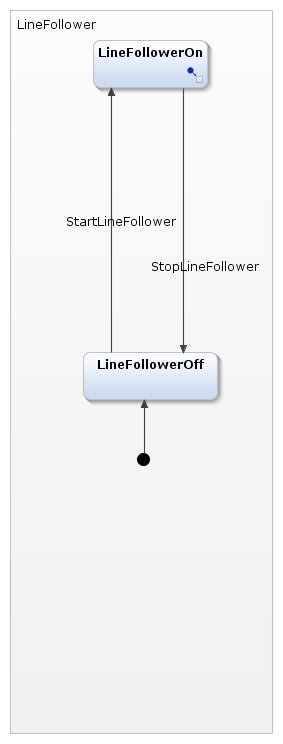
\includegraphics[scale=.7]{linefollower.png}
	\caption{line follower machine}
	\label{linefollower}
\end{minipage}
	\begin{minipage}{0.45\textwidth}
	\centering
	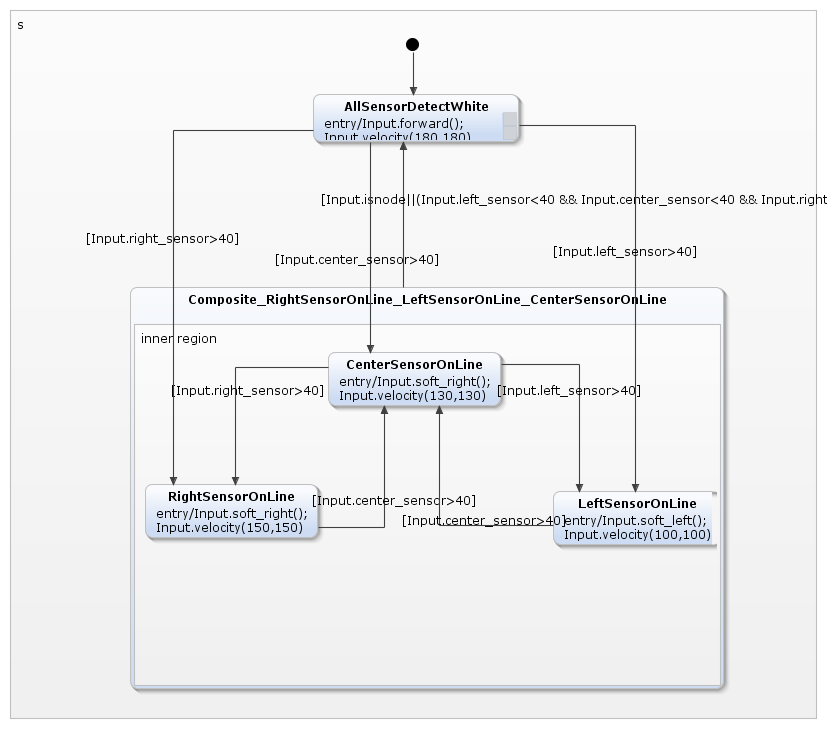
\includegraphics[scale=.6]{linefollower_on.png}
	\caption{LineFollowerOn state}
	\label{linefollower_on}
\end{minipage}
\end{figure}
It contains two states, \textit{LineFollowerOff} and \textit{LineFollowerOn} as shown in the figure \ref{linefollower}. Raising event \textit{StartLineFollower} when it is in \textit{LineFollowerOff} state makes transition to \textit{LineFollowerOn} state. 
The bot then starts following the line. Similarly, raising an event \textit{StopLineFollower} when it is in \textit{LineFollowerOn} state makes a transition to \textit{LineFollowerOff} and robot stops following the line.
The \textit{LineFollowerOn} state is further divided into some substates as shown in figure \ref{linefollower_on}. This state machine tries to follow the black line with the line between the left and center sensor. It contains states \textit{AllSensorsDetectWhite}, \textit{LeftSensorDetectLine}, \textit{CenterSensorDetectLine} and \textit{RightSensorDetectLine}. The actions are taken accordingly as the sensor values change after some threshold values.

\item \textbf{State machine for making turn}\\
It contains two states, \textit{TurningOn} and \textit{TurningOff} as shown in figure \ref{turn}. When robot needs to take a turn in the grid, we need to give value to a variable turn as \textit{left, right”, “back”} and \textit{forward} according to the needed turn. After that, we need to raise an event \textit{StartTurning}. Then it will enter the \textit{TurningOn} state. The robot will start turning. As the turn is completed, it will automatically go to the \textit{TurningOff} state.
\textit{TurningOn} state is further divided into further states as \textit{GoingForward, TurningLeft, TurningRight} and \textit{TurningBack} as shown in figure \ref{turning_on}.
The state which is entered is selected on the basis of corresponding value of the variable turn.
If system is in \textit{GoingForward} state, it will remain here and move forward. When the node is not detected i.e., the node has passed, it will exit this state and go to \textit{TurningOff} state.
	\begin{figure}[!htbp]
	\centering
	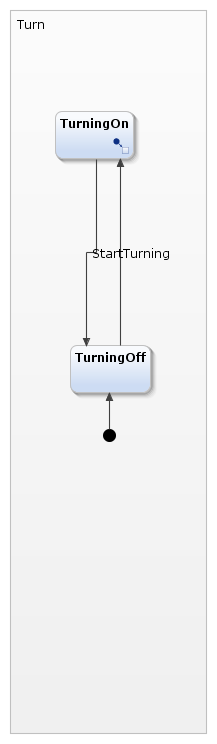
\includegraphics[scale=.6]{turn.png}
	\caption{Turn machine}
	\label{turn}
\end{figure}
\begin{figure}[!htbp]
	\centering
	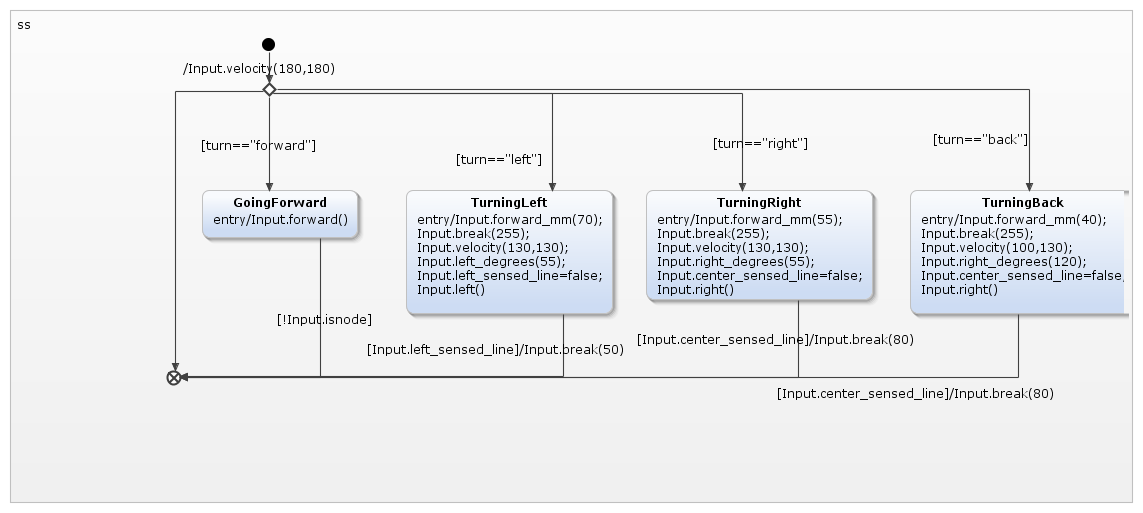
\includegraphics[scale=.65]{turning_on.png}
	\caption{TurningOn state}
	\label{turning_on}
\end{figure}

If system is in \textit{TurningRight} state, it will move bot forward 55 mm, break, move 55 degrees right and then keeps on turning right. When center sensor detects black (line), it will exit this state and go to \textit{TurningOff} state.
If system is in \textit{TurningLeft} state, it will move forward 70 mm, break, move 55 degrees left and then keeps on turning left. When left sensor detects black (line), it will exit this state and go to \textit{TurningOff} state.
If system is in \textit{TurningBack} state, it will move forward 40 mm, break, move 55 degrees right and then keeps on turning right with different velocities (to make sure of proper alignment with line as line should be between left and center sensor). When center sensor detects black (line), it will exit this state and go to \textit{TurningOff} state.

\item \textbf{Orientation state machine}\\
It keeps track of the orientation of the bot (figure \ref{orientation}). It contains four states \textit{East, West, North} and \textit{South}. It uses the turning state to orient the robot in a particular direction. 
\begin{figure}[h]
	\centering
	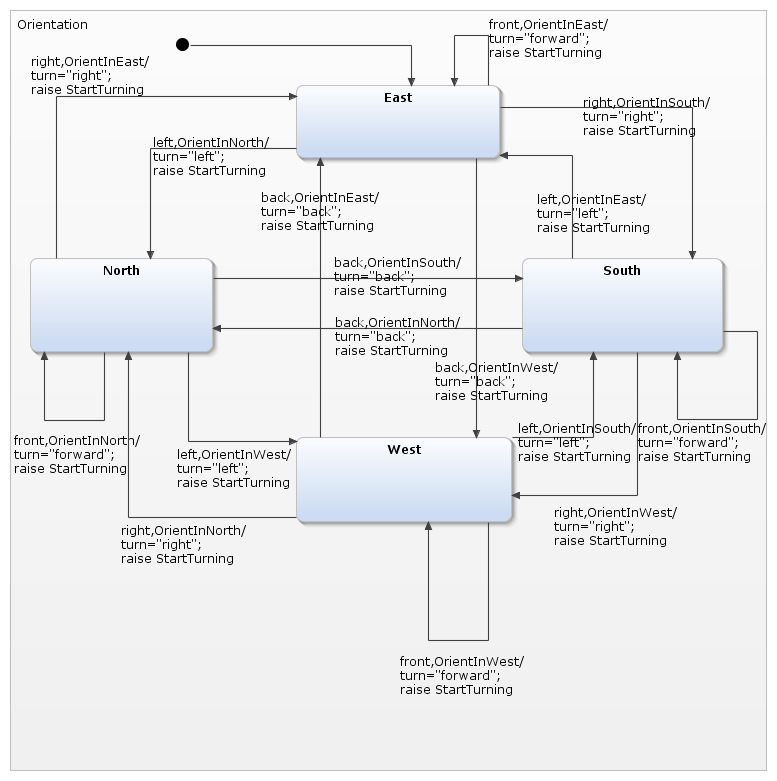
\includegraphics[scale=.6]{orientation.png}
	\caption{Orientation machine}
	\label{orientation}
\end{figure}
For example, if \textit{OrientInEast} event is raised, in whichever of the four state the system is, it will enter in \textit{East} state by using the turning state machine with proper turn. Another way of using this state machine is raising an event \textit{left, right, front} or \textit{back}. It will turn accordingly and update the orientation by going to the proper state.

\item \textbf{Coordinates state machine} \\
It contains only one state \textit{Coordinates} as shown in figure \ref{coordinates}. When an event \textit{update coordinates} is raised, it will update the $x$ and $y$ coordinates by incrementing or decrementing the appropriate value according to which of the state in Orientation state machine is active.
	\begin{figure}[]
		\begin{minipage}{0.45\textwidth}
	\centering
	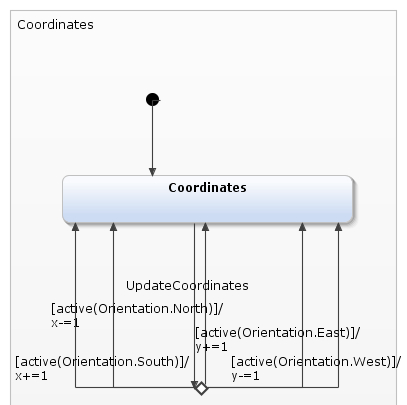
\includegraphics[scale=.6]{coordinates.png}
	\caption{Coordinates machine}
	\label{coordinates}
	\end{minipage}
\begin{minipage}{0.45\textwidth}
		\centering
	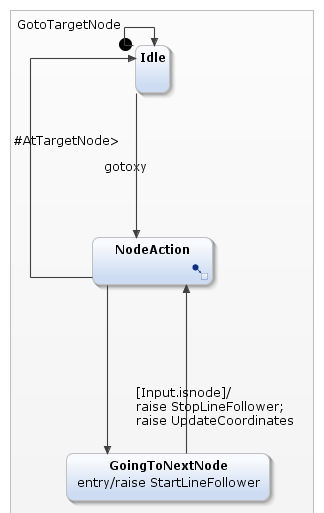
\includegraphics[scale=.6]{GoToTargetNode.png}
	\caption{GoToTargetNode machine}
	\label{GoToTargetNode}
\end{minipage}
\end{figure}
\begin{figure}[]
	\centering
	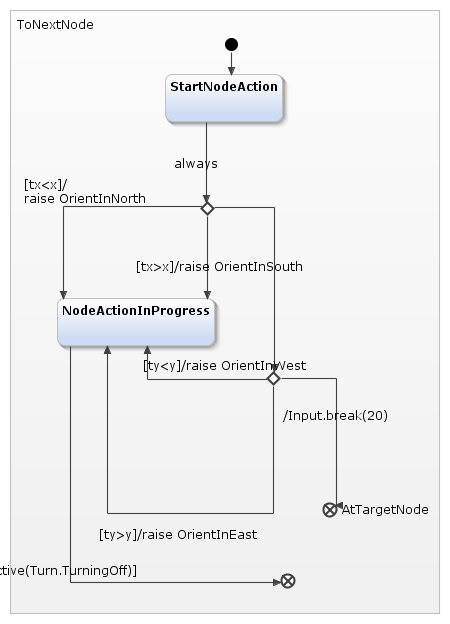
\includegraphics[scale=.6]{node_action.png}
	\caption{node action state}
	\label{node_action}
\end{figure}

\item \textbf{GotoTargetNode}\\
It takes the robot to the target node $tx$ , $ty$ (figure \ref{GoToTargetNode}). To use it, just give the values to $tx$ and $ty$. After that, raise an event \textit{gotoxy}. It will take the robot to the target coordinates in the grid. It contains substates 
	 \textit{Idle, NodeAction, GoingToNextNode} as shown in figure \ref{node_action}. 
\begin{enumerate}
\item  Idle state\\
When \textit{GotoTargetNode} is not being used, it remains in the \textit{Idle} state. When event \textit{gotoxy} is raised, it moves to \textit{NodeAction} state
\item NodeAction State\\
It takes the appropriate action at particular node for going to next node. If target node is reached, system goes to \textit{idle} state. Otherwise, first it checks whether the target $x$ is equal to present $x$ or not. If not, it moves the robot in $x$ direction. Otherwise, it checks whether the target $y$ is equal to the present $y$ or not. If not, it moves the bot in $y$ direction. When node action is being taken (turning in proper direction or moving out of the node), it remains in \textit{NodeActionInProgress} state. When the action is completed, it exits the \textit{NodeAction} state and goes to \textit{GoingToNextNode} state. When target node is reached, it will exit at \textit{AtTargetNode} exit point. 
\item \textit{GoingToNextNode} state\\
When system enters this state, it turns on the line follower. Robot starts following the line until the next node is reached. When next node is reached, it stops the line follower, updates the coordinates and goes to \textit{NodeAction} State.
\end{enumerate}
\item \textbf{Main}\\ 
It is \textit{main} state machine which uses all other state machines to accomplish the task (figure \ref{main}). Initially it enters start state and it starts the line follower. As a node is detected, line follower is stopped. The target coordinates are fetched from c function and event \textit{gotoxy} is raised.
	\begin{figure}[]
	\centering
	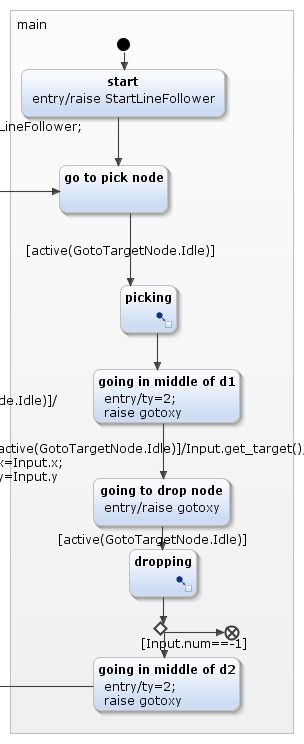
\includegraphics[scale=.8]{main.png}
	\caption{main machine}
	\label{main}
	\end{figure} 
Now it is in \textit{go to pick node} state. When the target node is reached, it enters \textit{picking} state (figure \ref{picking}). In \textit{picking} state, robot starts following the line and when some distance is reached, it picks the number. After a node is detected, it updates the coordinates, stops the line follower and exits the \textit{picking} state. It enters the \textit{going in middle of d1} state where it gives target coordinate as $ty$=2 and raises \textit{gotoxy} to reach to the middle of the grid d1. When it is reached, it gets next target coordinates and enters \textit{going to drop node} state. Here, it raises \textit{gotoxy}. The robot is now going towards drop node. When it reaches there, it goes to \textit{dropping} state (figure \ref{dropping}). This state is similar to \textit{picking} state except that it will drop the number at a certain distance. 
	\begin{figure}[]
	\begin{minipage}{0.45\textwidth}
	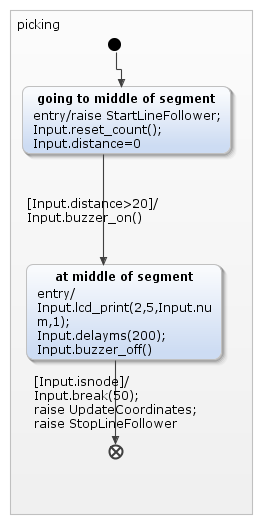
\includegraphics[scale=.6]{picking.png}
\caption{picking state}
\label{picking}
	\end{minipage}
\begin{minipage}{0.45\textwidth}
	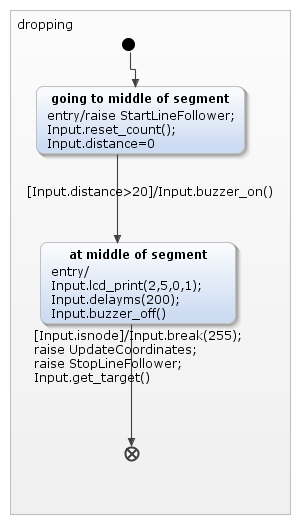
\includegraphics[scale=.6]{dropping.png}
\caption{dropping state}
\label{dropping}
\end{minipage}

\end{figure} 
After that, it gets next coordinates. If complete puzzle is solved (num==-1), it will exit the state machine. Otherwise, it will go to the \textit{going in middle of the d2}. After reaching in the middle of d2, it will go in \textit{go to pick node} state and the cycle repeats.

\pagebreak
\end{itemize}
\textbf{Stop state}\\
After complete puzzle is solved, system comes out of puzzle solver state and enters in this state where it stops and beeps a buzzer for 2 sec.
\\
\pagebreak
\section{Use and Demo }
Instructions for demonstration

\begin{enumerate}
	\item Open Atmel Studio 7.
	\item In main.c file, enter the sequence of numbers in d1 grid in "d1" array. Bottom left number should be entered first, then second number in the row and so on. after completing first row, move to the upper rows one by one.
	\item Enter the numbers present in grid d2 in 2d array "d2" where you need to add cell number and the number present in the cell for each number. Cell number starts from 0 at bottom left and increases as we move right and then on next row. Maximum of 4 numbers can be added in it. If you want to add less then 4 numbers, then fill \{-1,-1\} for the others.
	\item Compile the code and burn in the firebird V.
	\item Put the bot just ahead of start bar and start the bot. It will take some time to find the optimum solution according to how many numbers are entered. After that, it will start solving the puzzle and beep a long buzzer when the puzzle is solved.
	\begin{figure}[h]
		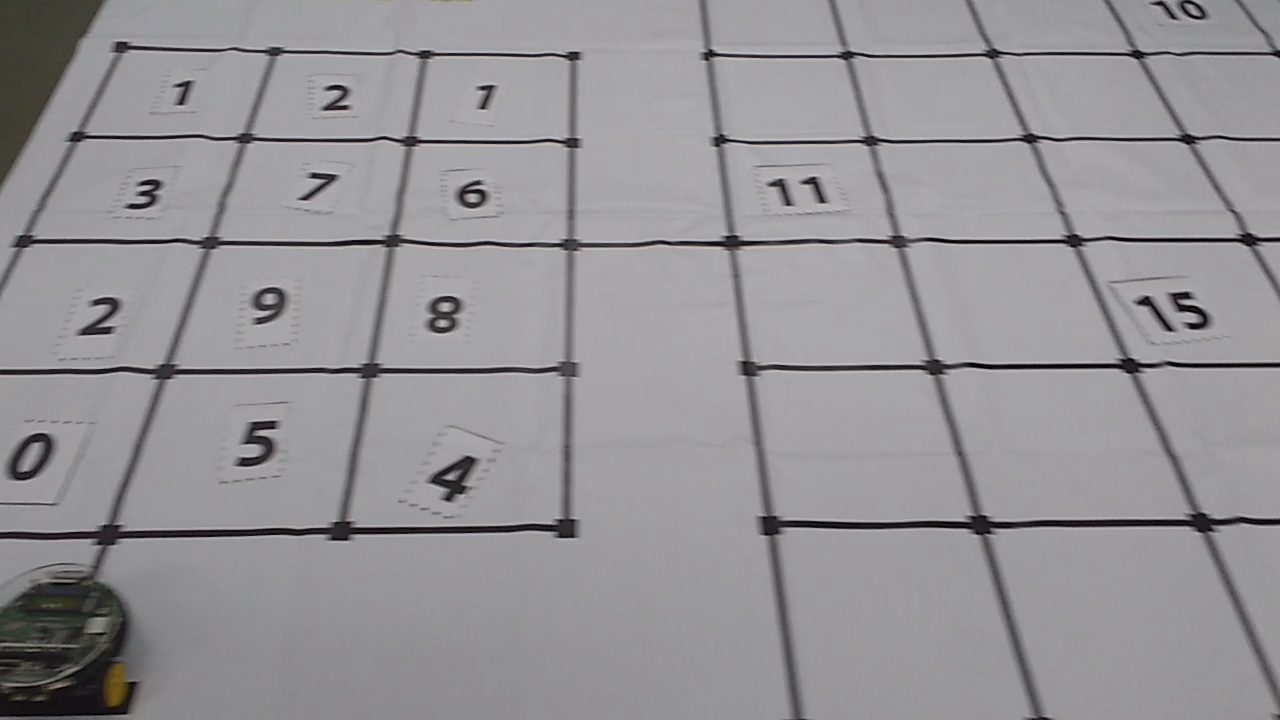
\includegraphics[scale=.3]{final_setup.png}
		\caption{final setup image}
	\end{figure}
	 
\end{enumerate}
\href{https://www.youtube.com/watch?v=SvR-iOOgiqY}{Youtube Link} of demonstration video 

\section{Future Work}
Inline simulation can be used for easy debugging in statecharts. By this feature, a developer may be able to see live which states are active as the code is running in real time. This feature may be of great help to developers to debug where things are going wrong.
\pagebreak
\section{Bug report and Challenges}
There is a bug in Yakindu SCT that if we copy any orthogonal region from one place and paste it in parallel with other regions then there is a problem that the sequence in which the control reaches the different states become ambiguous. This bug wasted too much time. Finally, step by step simulation was used to debug this unusual behavior. So, it is advisable that if you want to copy and paste any region, then instead of pasting directly, make a new orthogonal region and paste there all the sub states in it. This does not gives the problem of sequence.

One of the most important challenge faced was changing the perspective. Initially, I was thinking in terms of sequential programming rather than thinking in terms of concurrent executing state machines machines. This changing of perspective helped a lot in modeling the system as independent modules rather than a sequential flow of control from one state to another. 
\begin{thebibliography}{li}
\bibitem{1} David Harel, "Statecharts: A visual formalism for complex systems", \emph{Department of applied mathematics, The Weizmann Institute
	of Science, Rehovot, Israel}.
\bibitem{4} Kavi Arya, Blossom Coelho, Shradda Pandya, "A Model Based Approach to System Building Using the E-Yantra Educatonal Robot", \emph{Department of Computer Science, IIT Bombay}.
\end{thebibliography}


\end{document}

